%!TEX root = ../thesis.tex
%*******************************************************************************
%*********************************** First Chapter *****************************
%*******************************************************************************
\ifpdf
    \graphicspath{{Chapter1/Figs/Raster/}{Chapter1/Figs/PDF/}{Chapter1/Figs/}}
\else
    \graphicspath{{Chapter1/Figs/Vector/}{Chapter1/Figs/}}
\fi
\chapter{Introduction}  %Title of the First Chapter

Orangutans are unique among primates in that they are bimature and males show two distinct male morphs: the initial "unflanged" morph and the subsequent "flanged" morph \citep{Knott.2008}. Flanged males possess many secondary sexual characteristics that the unflanged male lacks, including a saggitial crest, a throat sac capable of making long calls, and fat cheek pads, also known as flanges \citep{Galdikas.1978cv}.

Although the development of these morphs in an individual is sequential, the unflanged form is not a "subadult" form, as they are sexually active and can cooperatively breed with females (though forced mating is more common) \citep{Knott.2009, Kunz.2023}. The transition between the two morphs can be arrested for many years, and in some habitats this transition can be arrested for decades \citep{Dunkel.2013}. 

Only recently have the mechanisms that trigger the development of the flange begun to be understood, which appears to be a mixture of social and endocrinological factors, including proximity to other flanged males and the presence of a stable local dominance hierarchy \citep{Dunkel.2013xnm, Marty.2015, Prasetyo.2019}.

Given that the transition from unflanged male to flanged male is irreversible, there remains debate about the plasticity of these traits after development, or whether their morphology is "fixed" during development. While throat sacs and associated long calls have been extensively studied in recent years, less attention has been paid to flanges and their plasticity after initial development \citep{Spillmann.2016}.

Physiologically, flanges are bilateral fleshy disc-shaped structures composed of fibrous connective tissue, adipose tissue, and muscle fibres \citep{Straus.1942,Winkler.1989}. These conspicuous features are believed to play a role in female mate choice, and are often used as part of individual identification \citep{Utami.2002km8, Kappeler.2004}

Various reports have been made from different field sites suggesting significant plasticity of the flange after development; however, the suggested causes or impacts of such a change have not yet been thoroughly investigated \citep{Galdikas.1978cv,Galdikas.1985, Knott.2009}.


The objectives of this dissertation are to:
\begin{enumerate}
    \item Quantify relative flange size using historic photographic data sets
    \item Examine how three key factors: age, fruit availability, and antagonistic male-male social interactions, shape the morphology of orangutan flanges after their development
    \item Examine shifts in behaviour from these individuals to estimate impacts or social correlates of reduced flange size
    \item Delve deeper into the cause(s) using long term behavioural data sets to gain wider insight into how this factor(s) shape flanged male behaviour
\end{enumerate}

By analysing two different populations in different species and ecologies, I hope to examine the role that social and nutritional factors play in the plasticity of these secondary sexual characteristics and provide greater insight into how these conspicuous traits impact, and are impacted, by their social and ecological environment.

\section{Structure of the dissertation}
This dissertation is split into 5 chapters. The first chapter is a general introduction to orangutans, their sexual dimorphism and bimaturism, and a short review of the limited articles that have observed this condition. 

The next three chapters are written as manuscripts for scientific papers. However, some of the methodology and data sets overlap between chapters, for example the facial landmarks measured in Chapter 2 form the basis of flange measurements from Chapter 3. 

In Chapter 2, I examine differences in fluctuating asymmetry in facial landmarks between sites using previously collected photographic data sets. I predicted that fluctuating asymmetry would be higher in the Bornean field site, and hypothesised that it was due to the differences in fruit availability in each site, the differential impacts of fire and historical human disturbance between sites.

In Chapter 3, I investigated the claim that the flange size varies over the lifetime of a flanged male. I predicted that due to the adipose content of the flanges, the reduction in the flange size would follow periods of low fruit availability. Additionally, I predicted that the psychoendocrinilogical factors that have been previously hypothesised to inhibit initial flange development would play a similar role after flange development; however, I predicted that this effect would be to a lesser extent than fruit availability. 

In Chapter 4, I investigate the impact of age on flanged male mating success and long call behaviour, including female association duration. I predicted a slow decrease in female association over time, in line with other primates; and that the energetic costs of long calls would be felt more strongly by older individuals leading to a change in their composition, frequency, or duration.

Finally, I conclude with Chapter 5, which summarises and synthesises the results from the main research chapters. 
\begin{figure}[htbp!] 
\centering    
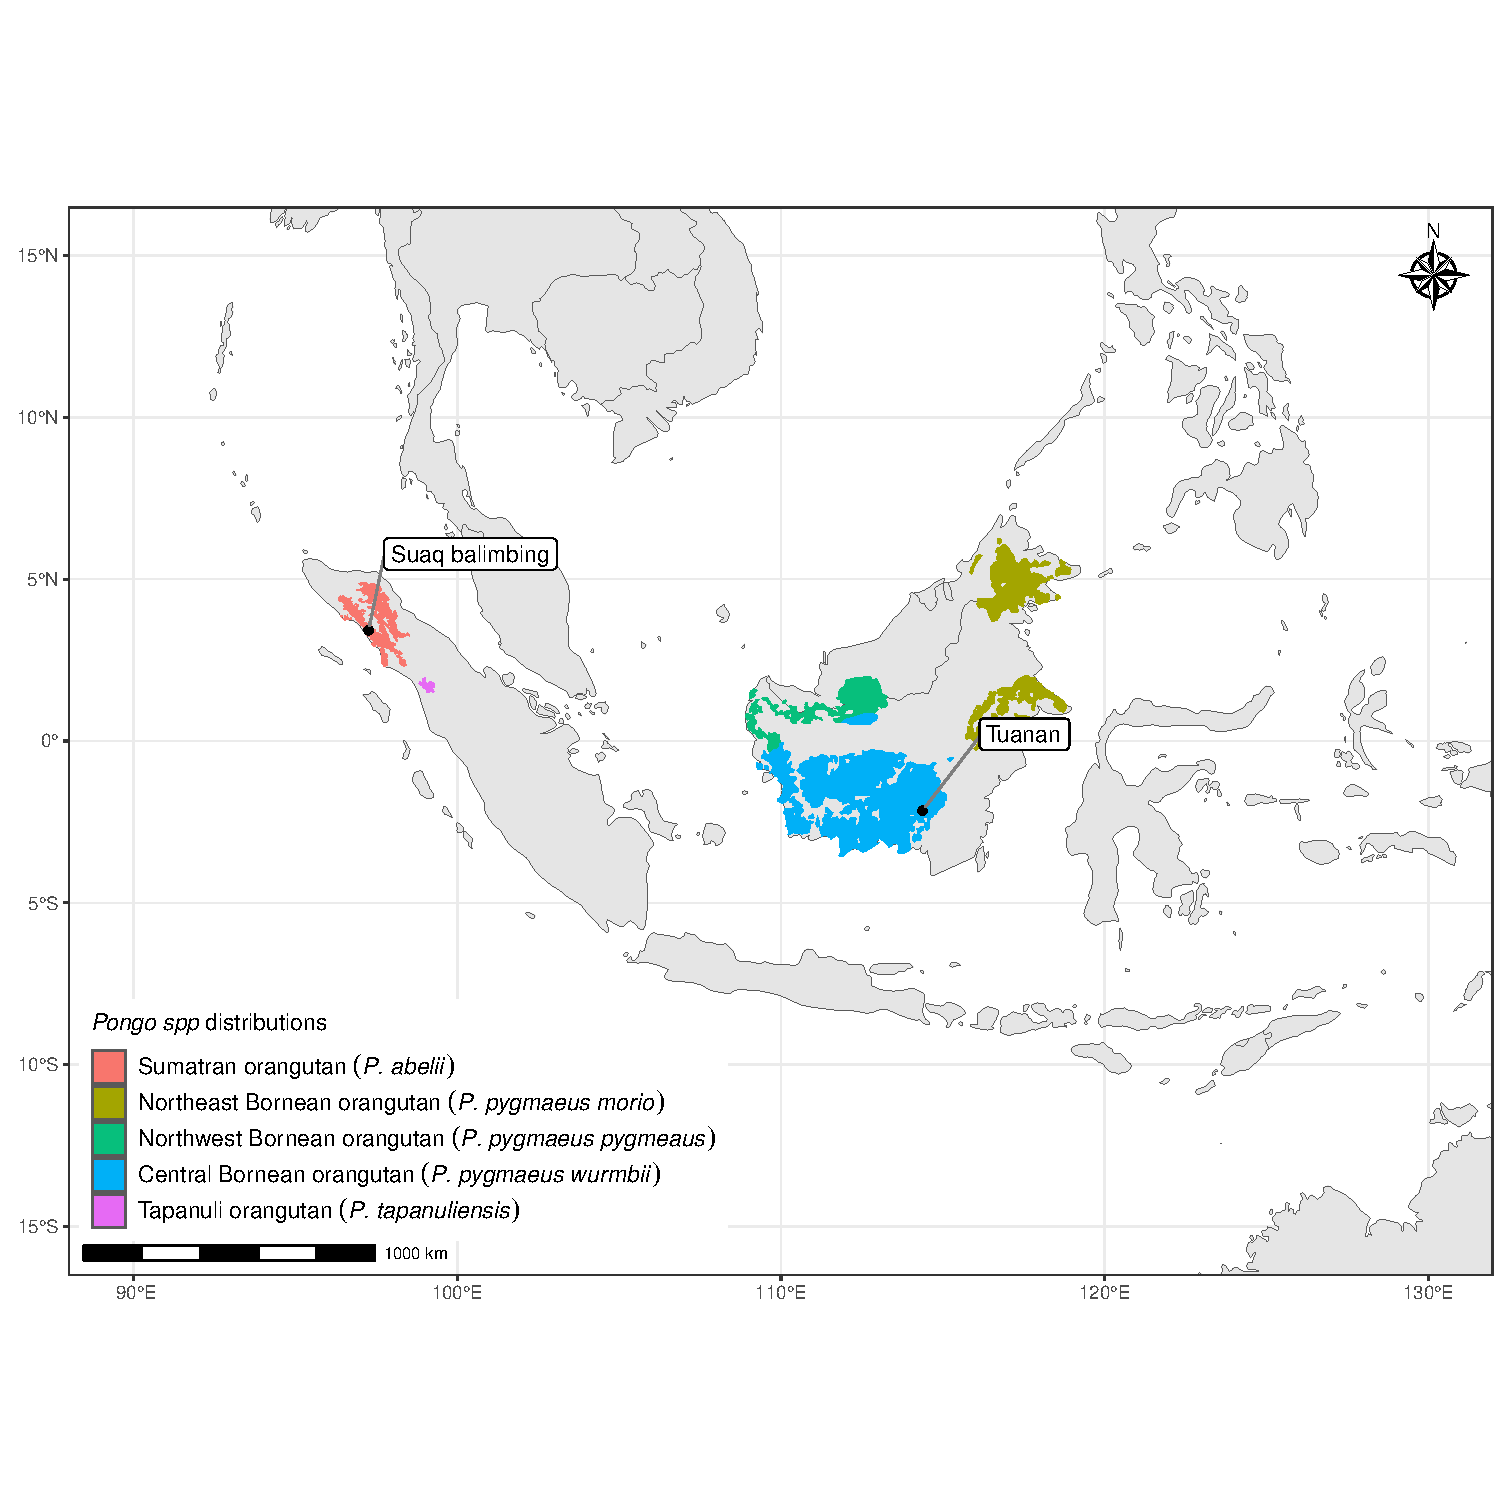
\includegraphics[width=1.0\textwidth]{mawasplot.eps}
\caption{Map illustrating orangutan distribution in Sumatra and Borneo. Locations of the field sites associated with the data in this dissertation are highlighted.}
\label{fig:A map of the distribution of wild Pongo spp. populations across Sumatra and Borneo, with the positions of Suaq Balimbing and Tuanan shown.}
\end{figure}


%********************************** %First Section  **************************************
\section{Introduction}
\subsection{Taxonomy \& distribution}
 %Section - 1.1 

Orangutans are the only extant members of the Ponginae sub-family, which split from the Homininae branch roughly 14 million years ago \citep{Grabowski.2017}. Their genus \textit{Pongo} originated 6 to 5 million years ago, and while historically members of the genus were found across mainland south-east Asia, since the late 1600s they are only located on the islands of Sumatra and Borneo \citep{Spehar.2018}.

The entire population was originally classified as a single species under the biological species concept, \textit{ Pongo pygmaeus}, despite the observed differences in morphology, behaviour, and ecology between Sumatran and Bornean populations. However, calls to have them classified as separate species grew in 1990s based on genetic evidence of species-level divergence between the two populations. Gel electrophoresis of isozymes and fibroblast proteins indicated indicated a split 1.5 million years ago between the Sumatran and Bornean populations, and mitochondrial DNA differences suggested a relatedness between the two species similar to that between horses and donkeys \citep{Janczewski.1990,Xu.1996}. These calls were officially recognised in 1999, when the Orangutan Action Plan officially recognised the Bornean orangutan (\textit{Pongo pygmaeus}) and the Sumatran orangutan (\textit{Pongo abelii}) as separate species \citep{Groves.1999}. 

This reclassification also recognised 3 subspecies of the Bornean orangutan based on their geographic position and multivariate analysis of their skull shapes and molars: 
\begin{itemize}
\item \textit{P. p. pygmaeus}, located in the north west of Borneo
\item \textit{P. p. wurmbii}, located in the south of Borneo
\item \textit{P. p. morio}, located in the north-east of Borneo in 2 separate patches
\end{itemize}

Finally, in 2017 the Tapanuli orangutan (\textit{Pongo tapanuliensis}), located only in the Batang toru ecosystem south of Lake Toba, was classified as a separate species based on its unique morphology, genetics and habitat; and is more closely related to the Bornean population than the Sumatran population only 400km north of them \citep{Nater.2017}. 
%********************************** %Second Section  *************************************

\section{Conservation status}
 %Section - 1.2

Great apes are particularly at risk to anthropogenic threats due to their nutritionally constrained dispersal ability, low population density, poor thermoregulation, and slow life history \citep{Carvalho.2019}. These factors are particularly noticeable in orangutans, for whom a 1\% population loss can drive a population to extinction \citep{Wich.2008}. Even under ideal conditions, an orangutan population can only grow in size by 2\% annually, and currently all orangutan populations are declining \citep{Utami-Atmoko.2016}.

All species of orangutan are currently classified as "Critically endangered" by the IUCN Red List and all have declining population trends. Current estimates of their population can be seen in Figure 1.2.

\begin{table}
    \centering
    \resizebox{\textwidth}{!}{%
\begin{tabular}{l c c c c r }
\hline 
\multirow{2}{*}{\textit{Pongo spp.}} & \multicolumn{4}{c}{Population Size}  & \multirow{2}{*}{References}\\ 
\cline{2-5}
  & Wild & Rehab.  & Zoo & Total (Estimated) \\ 
\hline
\textit{P. abelii} & 13,000 - 14,000 & Unk. & 319  & 13,319 - 14,319 &  \citep{Wich.2016, Utami-Atmoko.2016, na8}\\

\textit{P. pygmaeus morio} & 3,000 - 4,500 & Unk. & < 616  & 3,000 - 5,116 & \citep{Utami-Atmoko.2016, na8} \\\


\textit{P. pygmaeus pygmaeus} & 10,000 - 11,000 & Unk. & < 616 & 10,000 - 11,616 & \citep{Utami-Atmoko.2016, na8}\\

\textit{P. pygmaeus wurmbii} & 34,000 - 35,000 & Unk. & < 616 & 34,000 - 35,616 & \citep{Wich.2016, na8}\\

\textit{P. tapanuliensis} & < 800 & Unk. & Unk. & < 800 &\citep{Nater.2017, Laurance.2020, na8}\\
\hline 
\end{tabular}
}
\caption{Population estimates of orangutan species and sub-species. Zoo population estimates are based on the 2022 International Studbook of the Orangutan \citep{na8}.}
\end{table}

Orangutan spp. originated around 3 million years ago around the foothills of the Himalayas \citep{Rijksen.1999}. They are believed to have spread across the foothills of mountain ranges through South East Asia to the Sunda islands of Borneo, Sumatra, and Java \citep{Meijaard.2022}. As humans spread across this area, their population growth, slash and burn agriculture, hunting pressure, and environmental changes limited the range of orangutans to only two islands \citep{Rijksen.1999}. Today, the main threats to all species of orangutans are land use change, the illegal pet trade, and illegal hunting \citep{Rijksen.1999}. Palm oil plantations are a significant threat to surviving intact forest fragments and remain a major source of new land for plantations despite calls for industry reform. It is estimated that more than 50\% of Indonesian forest were lost to palm plantations between 1990 and 2005 \citep{Gibbs.2010}. Primary forests in carbon-rich peatlands are cleared to make room for palm oil plantations, which directly impacts the climate as well as biodiversity \citep{Gaveau.2009}. 40\% of palm oil in Indonesia and Borneo is produced by small landholders, whose disparate monocultures increasingly fragment existing orangutan populations, reducing the size of sub-populations to unviability \citep{Wich.2008v8i0d}. Of the estimated 100,000 orangutans that were killed between 1999 and 2015, most are estimated to have been killed due to selective logging in primary forests, as opposed to forest clearing or direct human-wildlife conflict \citep{Voigt.2018}. 

The Tapanuli orangutan faces a specific immediate threat due to the construction of a hydro-dam that is being constructed in the only intact forest patch currently connecting the three sub-populations \citep{Nater.2017,Laurance.2020}. The project, which is being implemented by Sinohydro as part of the Belt and Road Initiative, is highly politicised within Indonesia and many senior orangutan researchers who have been vocally critical of the project have been banned from conducting any further research in Indonesia \citep{Pramono.2022,CNN.2022}. Current projections estimate that construction will drive 2 of the sub-populations to unviability \citep{Wich.2019}. The third sub-population may remain viable, provided that planned logging concessions and gold mine expansion are not carried out, and all deforestation and orangutan killings stop permanently in the region \citep{Laurance.2020}. Defenders of the project propose the development of ecological corridors between the remaining sub-populations as a mitigation strategy, however, critics claim that there is currently a lack of evidence as to whether orangutans will use these corridors and question their effectiveness in linking the surviving sub-populations \citep{Kuswanda.2022}.

%********************************** % Third Section  *************************************
\section{Life history}  %Section - 1.3 

\label{section1.3}

Orangutans have the slowest life history of any great ape (except humans), with an inter-birth period of around 8 years \citep{Wich.2008t6}.  As arboreal primates with large home ranges and live forests characterised by a wide variation in food availability, acquiring ecological competence quickly is essential \citep{Noordwijk.2018}. Juveniles spend all of their time within 100m their mother until the age of 6-8 years, from whom they learn the majority of their skills through peering behaviour \citep{Wich.2008t6}. Following lactation, the ability of the female to conceive again is driven by the high availability of fruits so that they can reach the necessary physical condition \citep{Spillmann.2016}. Mothers adjust their own diet based on the ecological competence of their child and their ability to process specific foods, allowing the offspring to maximise opportunities for learning \citep{Mikeliban.2021}. Orangutans are mainly frugivorous, and fruits comprise the majority of their diet when available \citep{Galdikas.1988}. However, they are opportunistic feeders and also eat leaves, bark, pith, insects, small vines, and honey \citep{Galdikas.1988}. On rare occasions, males have been observed eating slow lorises in both Sumatra and Borneo \citep{Hardus.2012, Makur.2022}.

In addition to acquiring food, offspring need to learn how to build nests that orangutans generally create daily \citep{Prasetyo.2008}. Individuals from different areas show cultural modifications in their nest building behaviour, including covers and "pillows" \citep{Russon.2007}. Orangutans have been shown to carry specific leaves for hours to use them as part of their nest for that evening \citep{Russon.2007}. Due to orangutan female philopatry, juveniles show sex-specific attention biases as they age. Females target the majority of their peering behaviour towards their mother, however male juveniles spend a larger proportion of time peering at other individuals \citep{Ehmann.20216zj}. This is suggested to be in preparation for later ranging behaviour after the males reach independence.  Between the ages of 8-12, adolescents spend their time within their mothers home range, but living independently \citep{Wich.2008v8i0d}. After this period, male orangutans disperse in search of a new home range \citep{Morrogh-Bernard.2011zwh}. It is still unknown how far male orangutans travel, or for how long, but this ranging behaviour allows male orangutans to act as cultural vectors, spreading behaviours across sub-populations \citep{Mörchen.202378o}. Females acquire a new home range adjacent to their mothers and remain there for the rest of their life \citep{Wich.2008v8i0d}.  Unlike other great apes, orangutans are semi-solitary (due to the fluctuations in food availability) and their level of day-to-day socialisation depends on their population density, life stage, sex, and environment \citep{Wich.2008t6}. 

\section{Bimaturism and orangutan male morphs}
\subsection{Bimaturism}
Male orangutans are bimature \textit{ie} there are two sexually active male morphs capable of siring children: the flanged male and the unflanged male \citep{Galdikas.1985}. This is unique among primates, even though some primate species show different male morphs, such as the mandrill, these changes are reversible, and the "immature" form is not a case of arrested development \citep{Setchell.2001}. Interestingly, in some sites the transition from unflanged to flanged can be arrested for decades and the proportion of flanged males to unflanged males varies according to the local ecology of the site \citep{Dunkel.2013xnm, Kunz.2023}. \citet{Pradhan.2012} suggests part of the reason why elongated development arrest is not seen in other species more commonly is that it requires a very low adult mortality rate to be an evolutionary stable strategy.  

The ultimate causes of the differences between individuals in the timing of bimaturism are due to the evolutionary costs and benefits of becoming a flanged male: Increases in intrasexual competition vs. increases in perceived attractiveness. In Sumatra, population densities of orangutans are generally higher due to decreased variability in fruit availability and higher overall fruit production. This, in turn, reduces average home range sizes as there is reduced need to range widely for food, increasing the potential for males to monopolise access to females. This results in more stable dominance hierarchies, which increases the relative cost for an unflanged male to become flanged. However, when dominance hierarchies are unstable, the best strategy is to maximise the number of copulations, and as flanged males can easily defeat unflanged males we find a higher proportion of flanged orangutans under these conditions.

Although the evolutionary strategy for bimaturism is well accepted, the proximate triggers for bimaturism are not fully understood. The nutritional state does not appear to play a role in the initiation of the transition, as individuals with negative energy balance can still undergo the change \citep{Prasetyo.2021}. A hypothesis for how the transition is arrested is due to the psychoendoneuroligcal impact of social interactions that cause persistent stress in orangutans, suppress testosterone and increase cortisol levels \citep{Kingsley.1982}. \citet{Thompson.2012} found that testosterone levels in captive flanged males that had undergone developmental arrest were significantly lower than in males who had not, which may be an indication that early life testosterone levels predict the timing of bimaturism, but could also be due to an increase in testosterone levels after this transition. These results were reinforced by studies on wild orangutan males that showed a significant increase in testosterone metabolites in faecal samples in flanged males compared to unflanged males \citep{Marty.2015rzq}. However, this study did not find a significant difference in cortisol metabolite levels between the two morphs, which would be expected under the hypothesis. \citet{Marty.2015} suggests these results may be due to a stress avoidance strategy on the part of unflanged males to avoid conflict and that flanged males experience greater levels of competition, increasing their cortisol levels. \citet{Prasetyo.2021} found in a study of captive male orangutans that flanged males actually had the highest cortisol levels, compared to unflanged and developing males, but these results may have been in large part due to the solitary captive housing of flanged males in the study and the difference in energy intake. Ultimately, the proximate causes triggering bimaturism remain unknown and due to the differences in hormonal profiles between captive and wild orangutans, a large-scale assay of hormonal metabolites on a wild population where social behaviour is well studied may be required to unpack the relationships between these factors.

\subsection{Unflanged males}
Unflanged males vary in size, with young adults having a body mass similar to females, while fully grown unflanged males have a body mass between females and flanged males \citep{Kralick.2021}. Although they lack the fully developed secondary sexual characteristics of the flanged male, unflanged males have fully developed testes and have successfully sired offspring in captivity and in the wild \citep{Utami.2002km8}.  Due to the lack of ability to make a long call, unflanged males use a "silent searching" mating strategy \citep{Knott.2008}. Compared to flanged males, they range significantly more to increase the chance of locating females, and occasionally travel together without antagonistic interactions \citep{Setia.2008}.  Due to the preference of females for flanged males, unflanged males often resort to forced copulation, a rarity among great apes \citep{Knott.2009y9d}. Females can employ mating strategies to negate the worst of these problems by staying in the vicinity of flanged males and approaching long calls to shake off persistent unflanged males \citep{Knott.2009}. Unflanged males generally move away from long calls upon hearing them, despite flanged males being generally tolerant to unflanged males in their vicinity \citep{Spillmann.2010}. 

\subsection{Flanged males}
Flanged males are approximately twice the size of females and possess several secondary sexual characteristics that the unflanged male lacks \citep{Prasetyo.2021}. Flanged males have more body hair, a sagittal crest, and distinctive cheek pads, known as flanges \citep{Galdikas.1978}. Flanged males use a "wait and call" mating strategy, attracting females to their location by producing long calls, distinctive vocalisations that travel up to 1km \citep{Knott.2008, Utami.2002km8, Prasetyo.2019}. Newly immigrated flanged males employ a "challenge calling" strategy, by calling much more frequently than existing males in order to establish their presence in an area \citep{Hayward.2018}. 

The flanges, which are bilateral discs on each side of the face, are the most conspicuous secondary sexual characteristic that male orangutans develop, which are primarily formed of fat deposits bound to fibro-fatty tissues \citep{Straus.1942}. Any additional function of the flange beyond an indicator of fitness is somewhat unknown; however, most hypotheses link the function of the flange to the long call. \citet{Galdikas.1983} suggested that the slightly concave shape of the flange allows the individual to better locate the source of other long calls, while \citet{Mitani.1985ak1m} suggested that the shape allows individuals to focus their call in a specific direction. Despite these hypotheses, the acoustic impact of the flange has not yet been methodologically tested.

Interactions between flanged males are rare despite their overlap in home ranges and density within the forest, which is likely due to the long calls acting as a spacing mechanism \citep{Spillmann.2016}. When flanged males do meet, their interactions are almost always aggressive, and although lethal violence is uncommon, these antagonistic interactions commonly result in injuries, including as severe as the removal of digits \citep{Setia.2008}.  

\subsection{The "past-prime" flanged male}
The term "past-prime" was first used to describe a flanged male in 1978, where \citet{Galdikas.1978} described a focal individual, named PP, at the Tanjung Puting Reserve as "past his prime". They noted that PP spent significantly less time ranging compared to other flanged males in the area, and habituated to the human observers relatively quickly compared to the other flanged males in the field site. PP was described as different from the other flanged males based on their "\textit{sunken wrinkles and diminished cheekpads}", and PP died one year after habituation. Galdikas described another male with a flange that had been found in the same condition a few years later \citep{Galdikas.1978}. The individual had died approximately 12 hours before observation based on the level of decomposition; however, due to their condition no behavioural changes were observed. 

Since then it has been reported at multiple field sites that some orangutans have flanges that are shrivelled or deflated in appearance, however there is some disagreement on the ultimate cause of the condition \citep{Knott.2009, Dunkel.2013}.  \citet{Knott.2009} also suggests that the primary cause is age, but hints at loss of dominance being also a causative factor. Changes in secondary sexual characteristics associated with loss of dominance are observed in other primates, as mandrills that have lost alpha status show a reduction in the extent of red sexual skin colouration \citep{Setchell.2001}. Knott stated that the "past-prime" male "\textit{display[s] greatly diminished cheek flanges, they give significantly fewer long calls, have significantly lower testosterone levels and energy expenditure, mate infrequently, are less aggressive toward other males, and are subordinate to prime males}". However, while Knott began initial research in this area, no peer-reviewed articles have been published on the condition so far \citep{Knott.2009b}.  \citet{Dunkel.2013} however suggests poor body condition caused by reduced food availability as a possible cause of the condition, citing the seasonal variation in fruit production experienced at a number of field sites. 

Despite these observations, no peer-reviewed paper has examined the causes or social implications of the condition. Additionally, whether this is a threshold condition or is instead reflective of general level of flange plasticity after their initial development, which may be reflective of multiple causative factors, is also unknown.